
%(BEGIN_QUESTION)
% Copyright 2011, Tony R. Kuphaldt, released under the Creative Commons Attribution License (v 1.0)
% This means you may do almost anything with this work of mine, so long as you give me proper credit

This P\&ID shows the controls for an incinerating flare, used to safely incinerate poisonous gas compounds from a chemical manufacturing process:

$$\includegraphics[width=15.5cm]{i0004rx01.eps}$$

Suppose one day the operators tell you that the temperature of the flare stack is registering lower than it should.  TIC-37 registers 1135 $^{o}$F when the setpoint is 1400 $^{o}$F.  According to the operators, this low-temperature condition has persisted steadily for the last several hours, with stack temperature drifting around the 1140 $^{o}$F mark.

\filbreak

Identify the likelihood of each specified fault in this process.  Consider each fault one at a time (i.e. no coincidental faults), determining whether or not each fault could independently account for {\it all} measurements and symptoms in this process.

% No blank lines allowed between lines of an \halign structure!
% I use comments (%) instead, so that TeX doesn't choke.

$$\vbox{\offinterlineskip
\halign{\strut
\vrule \quad\hfil # \ \hfil & 
\vrule \quad\hfil # \ \hfil & 
\vrule \quad\hfil # \ \hfil \vrule \cr
\noalign{\hrule}
%
% First row
{\bf Fault} & {\bf Possible} & {\bf Impossible} \cr
%
\noalign{\hrule}
%
% Another row
PCV-40 set too low &  &  \cr
%
\noalign{\hrule}
%
% Another row
Partial blockage in FT-38 &  &  \cr
%
\noalign{\hrule}
%
% Another row
Burner management system tripped (shut down) &  &  \cr
%
\noalign{\hrule}
%
% Another row
Low air supply pressure to FY-38b &  &  \cr
%
\noalign{\hrule}
%
% Another row
Air leak in solenoid SV-115 &  &  \cr
%
\noalign{\hrule}
%
% Another row
Solenoid SV-101 shut &  &  \cr
%
\noalign{\hrule}
%
% Another row
Solenoid SV-103 shut &  &  \cr
%
\noalign{\hrule}
%
% Another row
6 inch waste stream header line blocked &  &  \cr
%
\noalign{\hrule}
} % End of \halign 
}$$ % End of \vbox

Finally, identify the {\it next} diagnostic test or measurement you would make on this system.  Explain how the result(s) of this next test or measurement help further identify the location and/or nature of the fault.

\underbar{file i03487}
%(END_QUESTION)





%(BEGIN_ANSWER)

% No blank lines allowed between lines of an \halign structure!
% I use comments (%) instead, so that TeX doesn't choke.

$$\vbox{\offinterlineskip
\halign{\strut
\vrule \quad\hfil # \ \hfil & 
\vrule \quad\hfil # \ \hfil & 
\vrule \quad\hfil # \ \hfil \vrule \cr
\noalign{\hrule}
%
% First row
{\bf Fault} & {\bf Possible} & {\bf Impossible} \cr
%
\noalign{\hrule}
%
% Another row
PCV-40 set too low & $\surd$ &  \cr
%
\noalign{\hrule}
%
% Another row
Partial blockage in FT-38 & $\surd$ &  \cr
%
\noalign{\hrule}
%
% Another row
Burner management system tripped (shut down) &  & $\surd$ \cr
%
\noalign{\hrule}
%
% Another row
Low air supply pressure to FY-38b & $\surd$ &  \cr
%
\noalign{\hrule}
%
% Another row
Air leak in solenoid SV-115 & $\surd$ &  \cr
%
\noalign{\hrule}
%
% Another row
Solenoid SV-101 shut &  & $\surd$ \cr
%
\noalign{\hrule}
%
% Another row
Solenoid SV-103 shut &  & $\surd$ \cr
%
\noalign{\hrule}
%
% Another row
6 inch waste stream header line blocked &  & $\surd$ \cr
%
\noalign{\hrule}
} % End of \halign 
}$$ % End of \vbox

%(END_ANSWER)





%(BEGIN_NOTES)

\vskip 20pt \vbox{\hrule \hbox{\strut \vrule{} {\bf Virtual Troubleshooting} \vrule} \hrule}

This question is a good candidate for a ``Virtual Troubleshooting'' exercise.  Presenting the diagram to students, you first imagine in your own mind a particular fault in the system.  Then, you present one or more symptoms of that fault (something noticeable by an operator or other user of the system).  Students then propose various diagnostic tests to perform on this system to identify the nature and location of the fault, as though they were technicians trying to troubleshoot the problem.  Your job is to tell them what the result(s) would be for each of the proposed diagnostic tests, documenting those results where all the students can see.

During and after the exercise, it is good to ask students follow-up questions such as:

\begin{itemize}
\item{} What does the result of the last diagnostic test tell you about the fault?
\item{} Suppose the results of the last diagnostic test were different.  What then would that result tell you about the fault?
\item{} Is the last diagnostic test the best one we could do?
\item{} What would be the ideal order of tests, to diagnose the problem in as few steps as possible?
\end{itemize}

%INDEX% Basics, control loop troubleshooting
%INDEX% Process: incinerator (realistic P&ID shown)

%(END_NOTES)


